\renewcommand{\NomeBloco}{\emph{vref\_block}}
\newcommand{\NomeBlocoA}{vrefblock}
\renewcommand{\NomePTab}{tab_\NomeBlocoA}
\renewcommand{\NomeSTab}{tab_\NomeBlocoA2}
\renewcommand{\NomePFig}{fig_\NomeBlocoA}
\renewcommand{\NomeSFig}{fig_\NomeBlocoA2}
\renewcommand{\NomeTTab}{tab_\NomeBlocoA3}

\section{vref\_block}

O bloco \NomeBloco{} tem a finalidade de conter o bloco \emph{vref\_generator}, mais o bloco respons\'avel por gerar a corrente que o polariza. O bloco apresenta as definições de sinais de entrada e sa\'ida referidos na \autoref{\NomeSTab}.

\begin{table}[!h] 
\caption{Sinais do bloco \NomeBloco}
\label{\NomeSTab}
\centering
\begin{tabular}{ccl}

    \toprule
    Sinal & Tipo    & Descrição      \\
    \midrule \midrule
    V\_extra   & Saída   & Tensão de refer\^encia 1 \\
    \midrule
    Vref\_plus   & Saída   & Tensão de refer\^encia 2 \\
    \midrule
    Vref   & Saída   & Tensão de refer\^encia 3 \\
    \midrule
    Vref\_minus   & Saída   & Tensão de refer\^encia 4 \\
    \midrule
    Vref\_minus2   & Saída   & Tensão de refer\^encia 5 \\
    \midrule
    Vref\_minus3   & Saída   & Tensão de refer\^encia 6 \\
    \midrule
    Vref\_minus4  & Saída   & Tensão de refer\^encia 7 \\
    \midrule
    Vref\_minus5   & Saída   & Tensão de refer\^encia 8 \\
    \midrule
    Vref\_minus6   & Saída   & Tensão de refer\^encia 9 \\
    \bottomrule
\end{tabular}
\legend{Fonte: Produzido pelo autor}
\end{table}

O circuito projetado para o bloco \'e demonstrado na \autoref{\NomePFig}.

\begin{figure}[htb]
 \centering
    \centering
    \caption{\label{\NomePFig}Circuito CMOS projetado para o bloco \NomeBloco}
    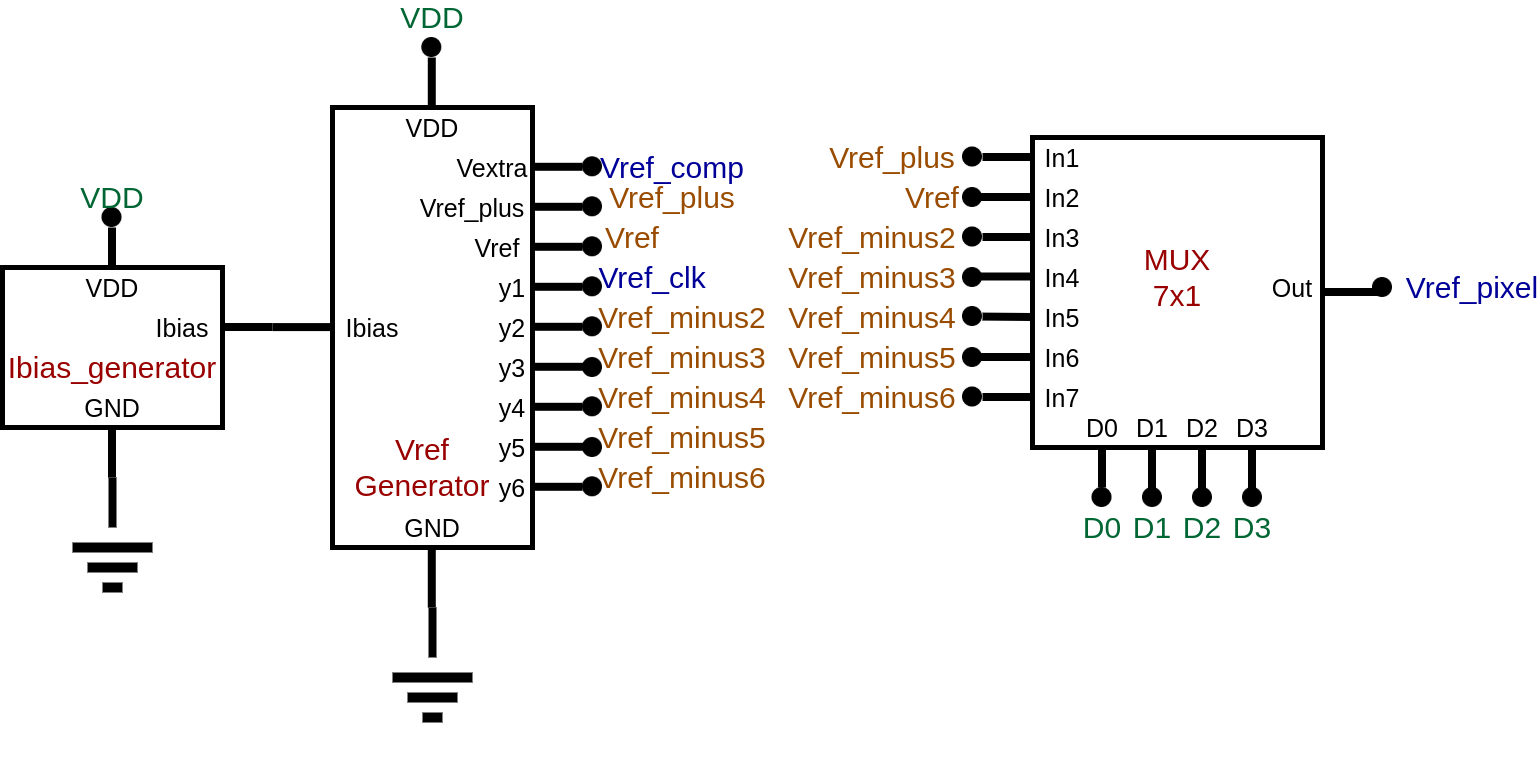
\includegraphics[scale=0.3]{Circuitos/vref_block.png}
    \legend{Fonte: Produzido pelo autor}
\end{figure}

\begin{figure}[htb]
 \centering
    \centering
    \caption{\label{\NomeSFig}Representação em bloco do \NomeBloco}
    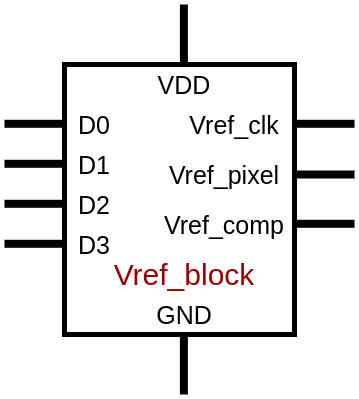
\includegraphics[scale=0.3]{Circuitos/vref_block_block.png}
    \legend{Fonte: Produzido pelo autor}
\end{figure}